\documentclass[titlepage]{article}
\usepackage{babel}
\usepackage{amsmath}
\usepackage{amssymb}
\usepackage{amsthm}
\usepackage{stmaryrd} %ligtning

\usepackage{tabto} %tabulator mit \tab
\usepackage{tikz}
\usetikzlibrary{automata, arrows.meta, positioning, shadows, shapes.geometric} % automaten zeichnen
\usepackage[utf8]{inputenc}
\pagestyle{plain}
\pagenumbering{arabic}
\renewcommand{\arraystretch}{1.3} %vertikaler abstand von tabellen
\usepackage[left=20mm, right=15mm, top=25mm, bottom=7mm, paper=a4paper]{geometry}

\renewcommand{\contentsname}{Inhaltsverzeichnis}
\renewcommand{\]}{\right]}
\renewcommand{\[}{\left[}
\renewcommand{\)}{\right)}
\renewcommand{\(}{\left(}
\renewcommand{\|}{\;|\;}
\newcommand{\n}{\newline}
\renewcommand{\l}{\linebreak}



\begin{document}\begingroup\let\clearpage\relax
	%header
	\begin{center}
	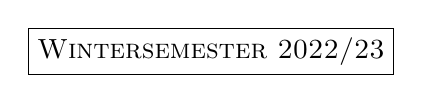
\begin{tikzpicture}
		\draw (0,0) node[draw, rectangle]{\textsc{Wintersemester 2022/23}};
	\end{tikzpicture}
	\hrulefill\\
	\begin{center}
		\LARGE\textsc{Automaten und Berechenbarkeit - Übung 04} \normalsize\\
	\end{center}
	\hrulefill
	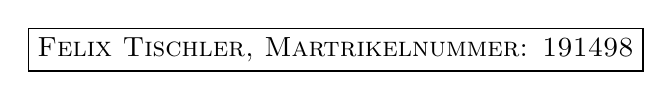
\begin{tikzpicture}
		\draw (0,0) node[draw, rectangle]{\textsc{Felix Tischler, Martrikelnummer: 191498}};
	\end{tikzpicture}
	\date{\today}
\end{center}
	
	%task one
	\paragraph{Aufgabe 1} Untersuchen Sie, ob die folgenden Sprachen über $\{a,b\}$ bzw. $\{a,b,c\}$ kontextfrei sind:
		\paragraph{(a)} $L_1=\{w\mid w\in\{a,b,c\}^*,\#_a(w)<\#_b(w)<\#_c(w)\}$
		\begin{align*}
	G_1=(\{a,b,c\},\{S,A,B,C, K\},S,R)&&&&&&&&&&&\\
	\text{mit }R:
	\begin{cases}
		S&\rightarrow bKc\mid aA\mid a\mid b\mid c\mid\lambda\\
		K&\rightarrow bK\mid Kc\mid b\mid c\\
		A&\rightarrow aA\mid bBc\\
		B&\rightarrow bBc\mid bc \\
	\end{cases}
\end{align*}
Initial wird entschieden ob $a$ in dem Wort auftreten oder nicht. Wenn dies der Fall ist, dass $a$ auftritt, dann muss $j=k$ sein. Hierfür ist das Nichtterminal $A$ vorgesehen. In $A$ können noch beliebig viele $a$ hinzugefügt werden, bis man über geht in das erzeugen des ersten $bc$. $b$ und $c$ werden immer zusammen erzeugt und dies beliebig oft. Man kann mit den Nichtterminalen $bc$ das Wort dann irgendwann beenden und hat die Bedingung $j=k$ sichergestellt. Sollte hingegen $a$ überhaupt nicht vorkommen, so spielt es keine Rolle wie oft $b$ und $c$ auftreten. Hierfür ist das Nichtterminal $K$ vorgesehen. In $K$ kann jeder Zeit mit $b$ oder $c$ beendet werden oder ein $b$ oder $c$ erzeugt werden. Die Spezialfälle sind in $S$ mit beachtet: Wenn $a$ nicht existiert kann direkt mit $b,c,\lambda$ beendet werden. Wenn $a$ mindestens einmal existiert kann auch direkt beendet werden.
		\paragraph{(b)}  $L_2=\{a^nb^mc^k\mid n,m,k\in\mathbb{N},n+m=k\}$
		Angenommen wir könnten es mit dem PL zeigen, dann müssten wir $x=uvw$ so wählen, dass wir zeigen können, dass $L\notin REG$. Hier wird es allerdings problematisch. Wir können $u$ nicht frei wählen. Dass einzige was wir aus dem PL wissen ist, dass $\mid uv\mid\le n$, somit muss unter den ersten $n$ Buchstaben unser $u$ sein. Da wir nun nicht eindeutig bestimmen können ob und wie oft $a,b,c$ in $u,v$ vorkommen können wir auch nicht wissen ob $a$ bspw. einmal vorkommt und somit $b$ aufpumpbar wäre um $\underbrace{j=k}_{\text{Siehe Def. $L$}}$ zu verletzten.\\\\Analog können wir auch jeden anderen Fall nicht kreieren in dem sich $L\notin REG$ mittels PL zeigen lässt. 
		\paragraph{(c)} $L_3=\{a^nb^mc^k\mid n,m,k\in\mathbb{N},n\cdot m=k\}$
		Ann: sei $L_3\in CF\Rightarrow\exists n\in\mathbb{N}:\forall x\in L_3\;mit\;\mid x\mid\ge n:\exists x=uv_1\tilde{v}v_2w\;mit\;\mid v_1v_2\mid\ge1,\mid v_1\tilde{v}v_2\mid\le n:\forall i\in\mathbb{N}:uv_1^i\tilde{v}v_2^iw\in L_3$:
\noindent\\\\
\begin{math}
	Wähle\;x=a^nb^nc^{n^2},\;mit\\\\
	u=a^{n-k_1-k_2-k_3}\\
	v_1=a^{k_1}\\
	\tilde{v}=a^{k_2}\\
	v_2=a^{k_3}\\
	w=b^nc^{n^2}\\
	mit\;k_1+k_2+k_3\le n\\\\
	\overset{i=0}{\Longrightarrow}a^{n-k_1-k_3}b^nc^{n^2}\Rightarrow L_3\notin CF
	\\\\Oder:\\\\
	u=a^n\\
	v_1=b^{k_1}\\
	\tilde{v}=b^{k_2}\\
	v_2=b^{k_3}\\
	w=c^{n^2}\\
	mit\;k_1+k_2+k_3=n\\\\
	\overset{i=0}{\Longrightarrow}a^nb^{k_2}c^{n^2}\Rightarrow L_3\notin CF
	\\\\Oder:\\\\
	u=a^nb^n\\
	v_1=c^{k_1}\\
	\tilde{v}=c^{k_2}\\
	v_2=c^{k_3}\\
	w=c^{n^2-k_1-k_2-k_3}\\
	mit\;k_1+k_2+k_3\le n\\\\
	\overset{i=0}{\Longrightarrow}a^nb^nc^{n^2-k_1-k_3}\Rightarrow L_3\notin CF
\end{math}\\
Man könnte auch noch in a und b oder in b und c pumpen, ebenso würde man durch pumpen ein nicht akzeptierbares Wort erhalten. 
		\paragraph{(d)} $A=\{0^n1^{n+m}0^m\mid n,m\in\mathbb{N},n>m>0\}$
		Ann: sei $A\in CF\Rightarrow\exists n\in\mathbb{N}:\forall x\in A\;mit\;\mid x\mid\ge n:\exists x=uv_1\tilde{v}v_2w\;mit\;\mid v_1v_2\mid\ge1,\mid v_1\tilde{v}v_2\mid\le n:\forall i\in\mathbb{N}:uv_1^i\tilde{v}v_2^iw\in A$:
\noindent\\\\
\begin{math}
	Wähle\;x=0^n1^{n+m}0^m,\;mit\\\\
	u=0^{n-k_1-k_2-k_3}\\
	v_1=0^{k_1}\\
	\tilde{v}=0^{k_2}\\
	v_2=0^{k_3}\\
	w=1^{n+m}0^m\\
	\;mit\;k_1+k_2+k_3\le n\\\\
	\overset{i=0}{\Longrightarrow}0^{n-k_1-k_3}1^{n+m}0^m\Rightarrow A\notin CF
\end{math}\\
Auch hier gibt es mehrere Möglichkeiten, wie bei (c) 
		\paragraph{(e)} $L_4=\{x\$y\mid x,y\in\{a,b\}^*,\#_a(x)=\mid y\mid\}$
		$G_2=(\{a,b\},\{S,R,K\},S,R)$
\begin{align*}
	Mit\;R=:
	\begin{cases}
		S&\rightarrow\quad aRa\mid aRb\mid bK\mid\$\\
		R&\rightarrow\quad bR\mid aRa\mid aRb\mid\$\\
		K&\rightarrow\quad aRa\mid aRb\mid bK\mid\$
	\end{cases}
\end{align*}
		\paragraph{(f)} $D=\{a^ib^jc^k\mid i,j\in\mathbb{N},i\neq j\}$
		$G_2=(\{a,b,c\},\{S,R,A,B,C\},S,R)$
\begin{align*}
	Mit\;R=:
	\begin{cases}
		S&\rightarrow\quad a\mid b\mid aRb\mid aC\mid bC\mid aA\mid bB\\
		R&\rightarrow\quad a\mid b\mid aRb\mid aC\mid bC\mid aA\mid bB\\
		A&\rightarrow\quad a\mid aA\mid aC\\
		B&\rightarrow\quad b\mid bB\mid bC\\
		C&\rightarrow\quad c\mid cC
	\end{cases}
\end{align*}
	
	\paragraph{Aufgabe 2} Konstruieren Sie einen Kellerautomaten, der die Sprache $\{w\in\{a,b\}^*\mid\#_a(w)=\#_b(w)\}$ akzeptiert.
	\newcommand{\nc[4]}{#2&#3&#4\\\hline}
\begin{center}
	$M=(\{0,1\},\{0,0_1,0_2,0_3,1,2,2_1,2_2,2_3,2_4,2_5\},\delta,\{0_1\},\{0_2,1,2,2_1,2_4\})$
	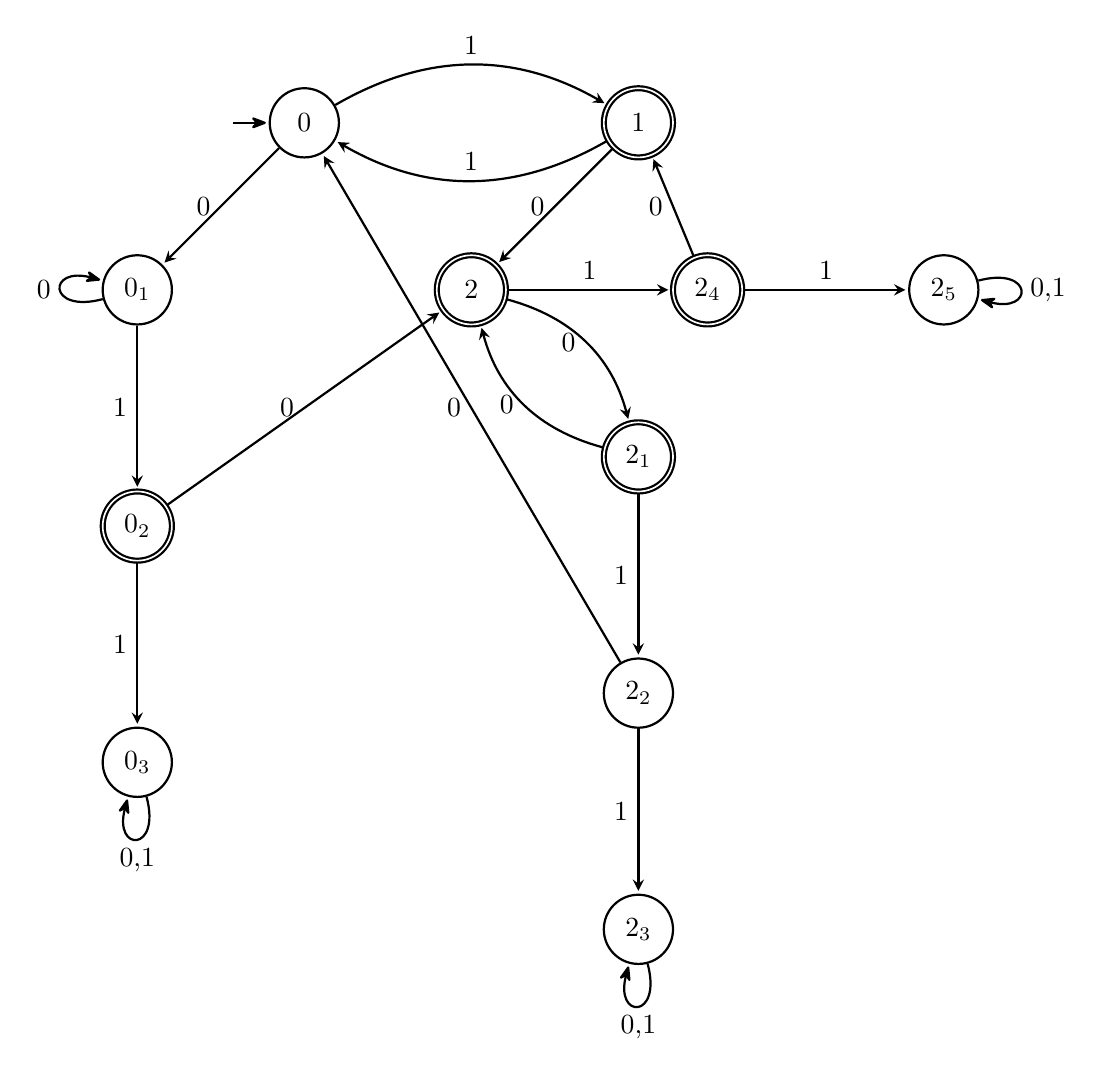
\begin{tikzpicture}[shorten >=1pt,node distance=3cm,on grid,>={Stealth[round]},thick]
		
		\node (q2) 
			[state, accepting] {2};
			\node (q21) 
				[state, accepting, below right of = q2] {$2_1$};
			\node (q22) 
				[state, below of = q21] {$2_2$};
			\node (q23) 
				[state, below of = q22] {$2_3$};
				
			\node (q24) 
				[state, accepting, right of = q2] {$2_4$};
			\node (q25) 
				[state, right of = q24] {$2_5$};
			
			
		\node (q0) 
			[state, initial, initial text = {}, above left of = q2] {0};
			\node (q01) 
				[state, below left of = q0] {$0_1$};
			\node (q02) 
				[state, accepting, below of = q01] {$0_2$};
			\node (q03) 
				[state, below of = q02] {$0_3$};
			
			
		\node (q1) 
			[state, accepting, above right of = q2] {1};
			
		
		
		\path [-stealth, thick]
		%(q0) edge [loop above] node [above] {$0$} (q0)
		(q0) edge [bend left] node [above] {1} (q1)
		(q0) edge node [left] {0} (q01)
		(q01) edge node [left] {1} (q02)
		(q02) edge node [left] {1} (q03)
		(q03) edge [loop below] node [below] {0,1} (q03)
		
		(q1) edge [bend left] node [above] {1} (q0)
		(q1) edge node [left] {0} (q2)
		
		(q2) edge [bend left] node [left] {0} (q21)
		(q21) edge [bend left] node [left] {0} (q2)
		(q21) edge node [left] {1} (q22)
		(q22) edge node [left] {1} (q23)
		(q22) edge node [left] {0} (q0)
		
		(q2) edge node [above] {1} (q24)
		(q24) edge node [above] {1} (q25)
		
		(q01) edge [loop left] node [left] {0} (q01)
		(q23) edge [loop below] node [below] {0,1} (q23)
		(q24) edge node [left] {0} (q1)
		(q25) edge [loop right] node [right] {0,1} (q25)
		(q02) edge node [left] {0} (q2)
		;
	\end{tikzpicture}
	
	$\delta:$
	\begin{table}[h]
		\centering
		\begin{tabular}{|c|c|c|}
			\hline
			Zustand & $0$ & $1$ \\
			\hline\hline
			\nc{$0$}{$0_1$}{$1$}
			\nc{$0_1$}{$0_1$}{$0_2$}
			\nc{$0_2$}{$2$}{$0_3$}
			\nc{$0_3$}{$0_3$}{$0_3$}
			\nc{$1$}{$2$}{$0$}
			\nc{$2$}{$2_1$}{$2_4$}
			\nc{$2_1$}{$2$}{$2_2$}
			\nc{$2_2$}{$0$}{$2_3$}
			\nc{$2_3$}{$2_3$}{$2_3$}
			\nc{$2_4$}{$1$}{$2_5$}
			\nc{$2_5$}{$2_5$}{$2_5$}
		\end{tabular}
	\end{table}
\end{center}
Der Automat ist folgendermaßen entstanden: Ich habe den Automaten der letzten Übungsserie genommen in dem beschrieben wird wann eine binär Zahl durch 3 teilbar ist:
\begin{center}
	$M_2=(\{0,1\},\{\equiv_3=0,\equiv_3=1,\equiv_3=2\},\delta_2,\{\equiv_3=0\},\{\equiv_3=0\})$\\
	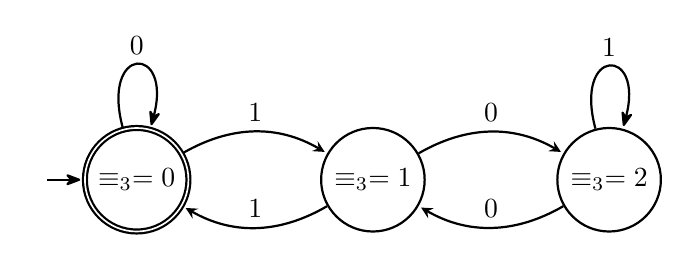
\begin{tikzpicture}[shorten >=1pt,node distance=3cm,on grid,>={Stealth[round]},thick]
		
		\node (q0) [state,initial, accepting, initial text = {}] {$\equiv_3=0$};
		\node (q1) [state, right of = q0] {$\equiv_3=1$};
		\node (q2) [state, right of = q1] {$\equiv_3=2$};
		
		\path [-stealth, thick]
		(q0) edge [loop above] node [above] {$0$} (q0)
		(q0) edge [bend left] node [above] {$1$} (q1)
		(q1) edge [bend left] node [above] {$1$} (q0)
		(q1) edge [bend left] node [above] {$0$} (q2)
		(q2) edge [bend left] node [above] {$0$} (q1)
		(q2) edge [loop above] node [above] {$1$} (q2);
		
	\end{tikzpicture}
	
	$\delta_2:$
	\begin{table}[h]
		\centering
		\begin{tabular}{|c|c|c|}
			\hline
			Zustand & $0$ & $1$ \\
			\hline\hline
			$\emptyset$&$\emptyset$&$\emptyset$\\
			\hline
			$\equiv_3=0$&\nm[$\equiv_3=0$]&\nm[$\equiv_3=1$]\\
			\hline
			$\equiv_3=1$&\nm[$\equiv_3=2$]&\nm[$\equiv_3=0$]\\
			\hline
			$\equiv_3=1$&\nm[$\equiv_3=1]$&\nm[$\equiv_3=2$]\\
			\hline
		\end{tabular}
	\end{table}
\end{center}
Von hier aus habe ich dann alle Fälle betrachtet in denen eine $0$ gelesen wird und habe diese dann zu einem dedizierten Zustand weitergeleitet. In jedem dieser Fälle habe ich dann betrachtet wie sich sowohl die Nicht-Teilbarkeit durch 3 verhält, als auch ob ein neuer Zustand benötigt wird um das Teilwort $011$ zu kapseln. Dieser Automat kann prinzipiell jedes Wort lesen. Wenn jedoch eine Sequenz $011$ auftritt, egal wo man sich vorher befunden hat, so  endet man in $0_3\lor2_3\lor2_5$. Somit ist wenn dieses Teilwort aufgetreten ist es nicht mehr möglich akzeptiert zu werden. In allen anderen fällen ist es möglich ein Wort zu lesen, dass akzeptiert wird, hierfür muss jedoch die Nicht-Teilbarkeit durch 3 gegeben sein. Dieses habe ich mittels dem Automaten der Übungsserie 4 abgeleitet. Jeder Zustand im Automaten besitzt neben der Information welche Zahlen vor ihm gelesen wurden auch die Information ob er durch 3 Teilbar ist oder nicht. Diese Informationen verteilen sich wie folgt: $0,0_1,2_2$ sind durch 3 teilbar. $1,0_2,2_1$ sind durch 3 Rest 1 teilbar und somit zu akzeptieren. Und $2,2_4$ sind durch 3 Rest 2 teilbar und folglich auch zu akzeptieren. 
	
	\endgroup\end{document}